\documentclass{article}
\usepackage{amsmath, amssymb, graphicx}
\usepackage[margin=1in]{geometry}
\usepackage{hyperref}
\usepackage[numbers,sort&compress]{natbib}
\usepackage{subfigure}
\usepackage{booktabs}
\usepackage{float}

\title{Progress Report: Efficient Trading with Price Impact}
\author{Jibran Bohra}
\date{\today}

\begin{document}
\maketitle

\section{Price Impact}
Price impact is the change in an asset's price caused by trading. In essence, price moves as a function of the signed volume $v$ (positive for net buys, negative for net sales). We study this relationship through an impact function $f$:
\begin{equation}
\Delta p = f(v).
\end{equation}
Understanding price impact helps estimate the hidden cost of trading, minimize execution costs, and reveal how markets absorb orders. This report documents the implementation and analysis of price impact models based on the paper ``Efficient Trading with Price Impact'' (ETwPI). 

\subsection{Data}
\subsubsection{Source and Sample}
We use an event-level limit order book dataset (MBO/MBP-1). Table~\ref{tab:first5_merged_data} shows the first five rows:
\begin{table}[ht]
\centering
\caption{First 5 rows of merged\_data.csv}
\label{tab:first5_merged_data}
\begin{tabular}{lrrrrrrr}
\hline
ts\_event & bid\_fill & ask\_fill & signed\_volume & price & best\_bid & best\_ask & mid\_price \\
\hline
2024-10-22 08:00:00 & 801.0 & 1999.0 & -1198.0 & 236.14 & 235.83 & 236.14 & 235.985 \\
2024-10-22 08:00:01 & 201.0 & 202.0 & -1.0 & 236.13 & 235.83 & 236.13 & 235.98 \\
2024-10-22 08:00:02 & 1600.0 & 1400.0 & 200.0 & 235.83 & 235.83 & 236.11 & 235.97 \\
2024-10-22 08:00:03 & 534.0 & 400.0 & 134.0 & 236.1 & 235.96 & 236.1 & 236.03 \\
2024-10-22 08:00:04 & 400.0 & 502.0 & -102.0 & 236.11 & 235.96 & 236.11 & 236.035 \\
\hline
\end{tabular}
\end{table}

\subsubsection{Preprocessing}
For each consecutive event we compute the price change and the elapsed time interval
\begin{align}
\Delta p_t &= \text{mid\_price}_t - \text{mid\_price}_{t-1},\\
\Delta t_t &= (\text{ts\_event}_t - \text{ts\_event}_{t-1})\;\text{in seconds}.
\end{align}
We drop missing values, keep realistic intervals \(0 < \Delta t_t < 60\) seconds, and remove \(\Delta p_t\) outliers beyond 3 standard deviations. We time-normalize signed volume to capture impact decay
\begin{equation}
X_t \;=\; \frac{v_t}{\sqrt{\Delta t_t}}.
\end{equation}

\subsubsection{Exploratory Data Analysis}
\begin{figure}[H]
\centering
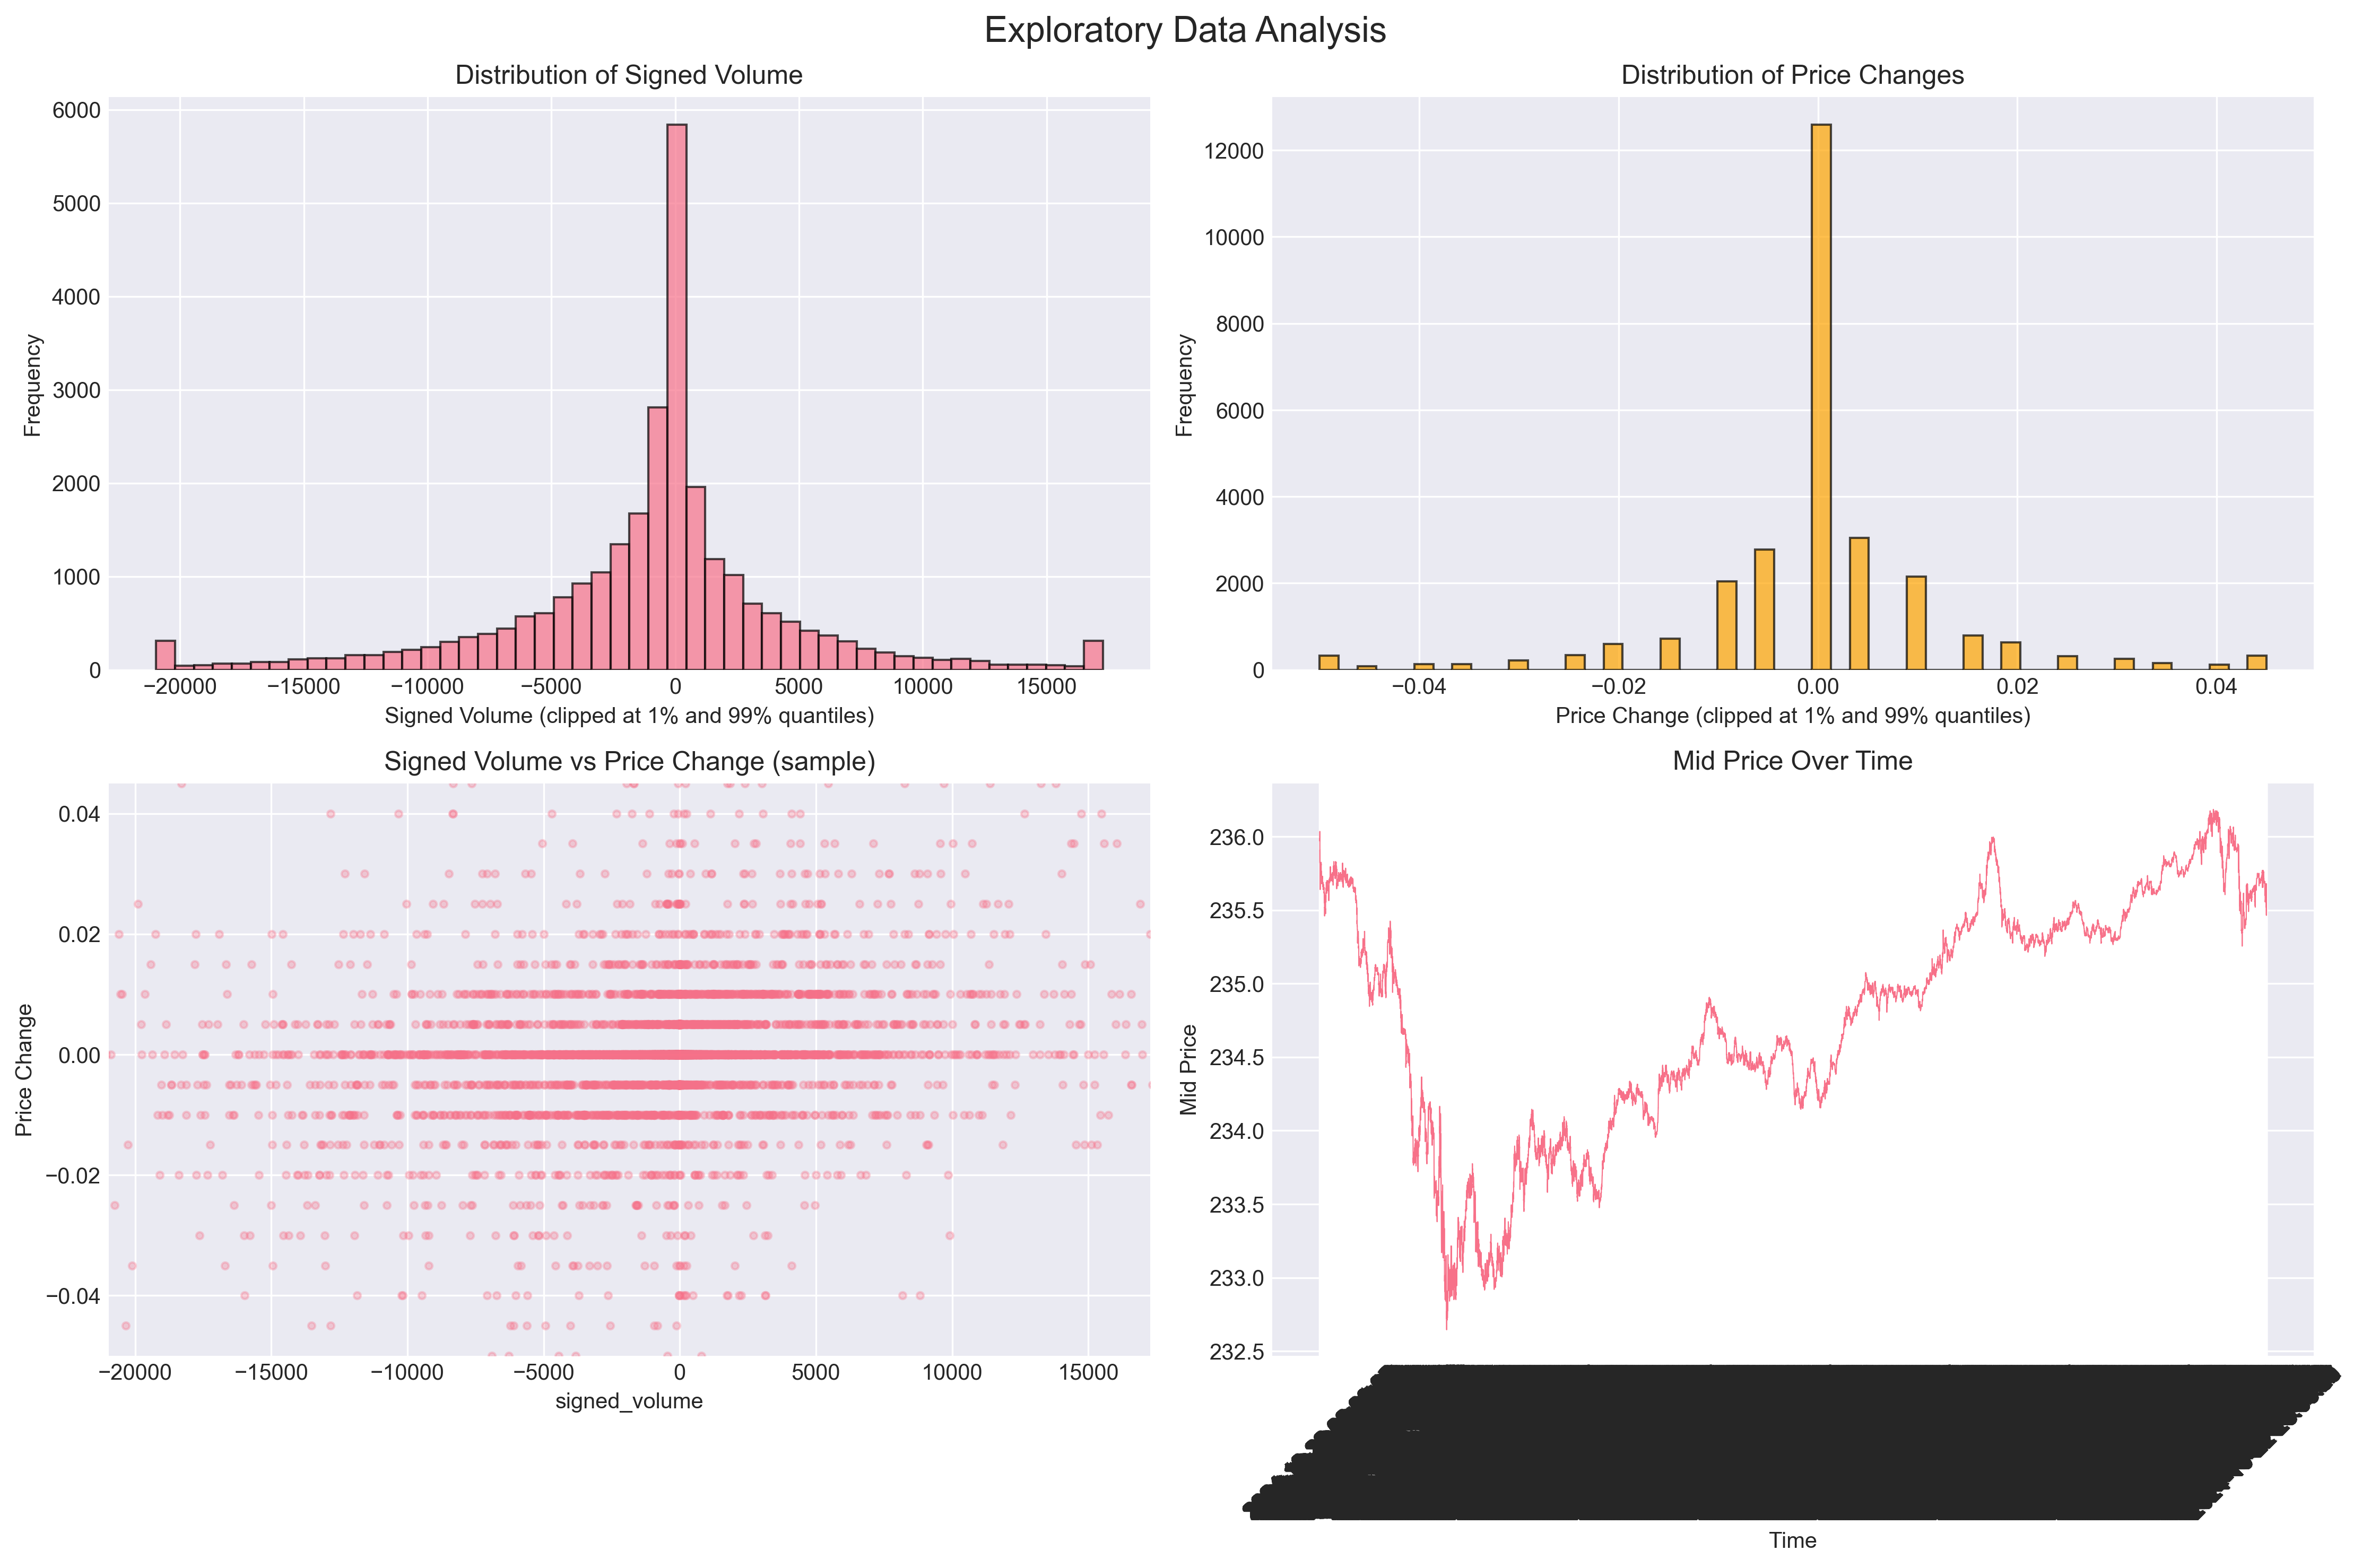
\includegraphics[width=\textwidth]{figures/01_exploratory_analysis.png}
\caption{Exploratory Data Analysis. Distributions of signed volume and price changes (clipped to 1\%--99\% quantiles) reveal heavy tails and a zero-centered return distribution; a 5{,}000-point sample scatter of $v$ vs. $\Delta p$ shows a weak but positive association; the mid-price series provides context for intraday dynamics.}
\label{fig:eda}
\end{figure}

\paragraph{Discussion.} Figure~\ref{fig:eda} reveals several microstructure regularities. In the \emph{top-left} panel, the signed-volume histogram is sharply peaked at zero with heavy tails, indicating many small trades punctuated by occasional large imbalances; the near symmetry suggests little directional bias on average. The \emph{top-right} panel shows price changes that are zero-centered and visibly quantized by the tick (and half-tick for the mid-price), producing a tall spike at zero and discrete mass at fixed increments. The \emph{bottom-left} scatter of $v$ versus $\Delta p$ exhibits horizontal banding from tick-size discreteness and vertical striations from discrete lot sizes; dispersion increases with $|v|$, consistent with a concave impact relationship as in Eq.~\eqref{eq:afs}, while any linear component appears weak. Finally, the \emph{bottom-right} mid-price series shows local trends and volatility clustering across the session. Taken together, these features motivate our preprocessing (time-normalizing volume by $\sqrt{\Delta t}$ and trimming outliers) and our emphasis on a nonlinear, concave impact specification.
\subsection{Models}
We successfully implemented two price impact models:

\begin{enumerate}
    \item \textbf{Linear Order-Weighted (OW) Model}: Assumes price impact is linear in order flow,
    \begin{equation}\label{eq:ow}
      \Delta p_t = \lambda \cdot \frac{v_t}{\sqrt{\Delta t}} + \epsilon_t.
    \end{equation}
    \item \textbf{Nonlinear Almgren-Fruth-Schied (AFS) Model}: Captures concave, nonlinear impact with a pure power-law response,
    \begin{equation}\label{eq:afs}
      \Delta p_t = \eta \cdot \operatorname{sign}(v_t) \cdot \left|\frac{v_t}{\sqrt{\Delta t}}\right|^\delta + \epsilon_t.
    \end{equation}
\end{enumerate}
where $v_t$ is the signed volume, $\Delta t$ is the time interval, and the division by $\sqrt{\Delta t}$ captures the temporal decay of price impact. Equations~\eqref{eq:ow} and~\eqref{eq:afs} highlight the key difference between the models: the OW specification is linear in time-normalized signed volume, whereas the AFS specification is concave due to the power-law term with exponent $\delta\in(0,1]$.


\paragraph{Linear OW fit.} The linear model regresses \(\Delta p_t\) on \(X_t\) using ordinary least squares with a closed-form estimator
\begin{equation}
\hat{\lambda} \;=\; \frac{\sum_t X_t\,\Delta p_t}{\sum_t X_t^2}.
\end{equation}
We report \(R^2\) and the number of samples retained after filtering.

\paragraph{Nonlinear AFS fit.} The nonlinear model uses a fixed exponent \(\delta\) (default 0.5) and a pure power-law impact without a linear term:
\begin{equation}
\Delta p_t \;=\; \eta\,\operatorname{sign}(X_t)\,|X_t|^{\delta} + \varepsilon_t.
\end{equation}
With $Z_t = \operatorname{sign}(X_t)\,|X_t|^{\delta}$, the single coefficient $\eta$ is estimated in closed form by ordinary least squares,
\begin{equation}
\hat{\eta} \;=\; \frac{\sum_t Z_t\,\Delta p_t}{\sum_t Z_t^2}.
\end{equation}
This works because for fixed $\delta$ the nonlinear transformation is applied to the \emph{regressor}, not the parameter: defining $Z_t$ maps the original specification to a one-parameter linear regression
\begin{equation}
\Delta p_t \;=\; \eta\, Z_t + \varepsilon_t, \qquad Z_t = \operatorname{sign}(X_t)\,|X_t|^{\delta}.
\end{equation}
Hence the model is linear in the unknown $\eta$ and OLS is an appropriate estimator under standard conditions (e.g., $\mathbb E[\varepsilon_t\mid Z_t]=0$ and finite conditional variance). If $\delta$ is unknown and to be estimated, the problem becomes nonlinear in parameters; common approaches are (i) profile OLS over a grid of $\delta$ values, selecting the $\delta$ that minimizes the residual sum of squares, or (ii) joint nonlinear least squares on $(\eta,\delta)$.
Goodness-of-fit is reported via $R^2$.


\subsection{Model Comparison and Visualization}
Figure~\ref{fig:detailed} summarizes how the models relate to the data across complementary views. In the \emph{top-left} panel, the hexbin density of observed $\Delta p$ against $v$ reveals tick-driven banding and increasing dispersion as $|v|$ grows; superimposed curves show the OW line cutting roughly through the center of the cloud while the AFS curve bends concavely, matching the widening spread for larger magnitudes. Near the origin both models are close, but as volume increases in either direction the AFS curve departs more strongly, consistent with diminishing marginal impact. The \emph{top-right} panel isolates this concavity by plotting the nonlinear component (AFS $-$ OW) in bps; the S-shaped, approximately odd-symmetric profile confirms small differences for modest $|v|$ and growing positive (negative) adjustments for large buys (sells). In the \emph{bottom-left} panel, predicted impact distributions for typical volumes show a narrow, sharply peaked OW distribution versus a broader AFS distribution with heavier shoulders, reflecting the latter's capacity to accommodate larger impacts at the tails while remaining conservative around zero. Finally, the \emph{bottom-right} metrics panel documents an improvement in $R^2$ when moving from OW to AFS, along with parameter estimates: a small but significant linear sensitivity in OW and, for AFS, an estimated $\eta$ with fixed $\delta=0.5$ that encodes concavity consistent with the microstructure patterns seen in the density plot. Together these views indicate that a concave response better captures how markets absorb larger order imbalances while preserving near-linear behavior for small trades.

\begin{figure}[H]
  \centering
  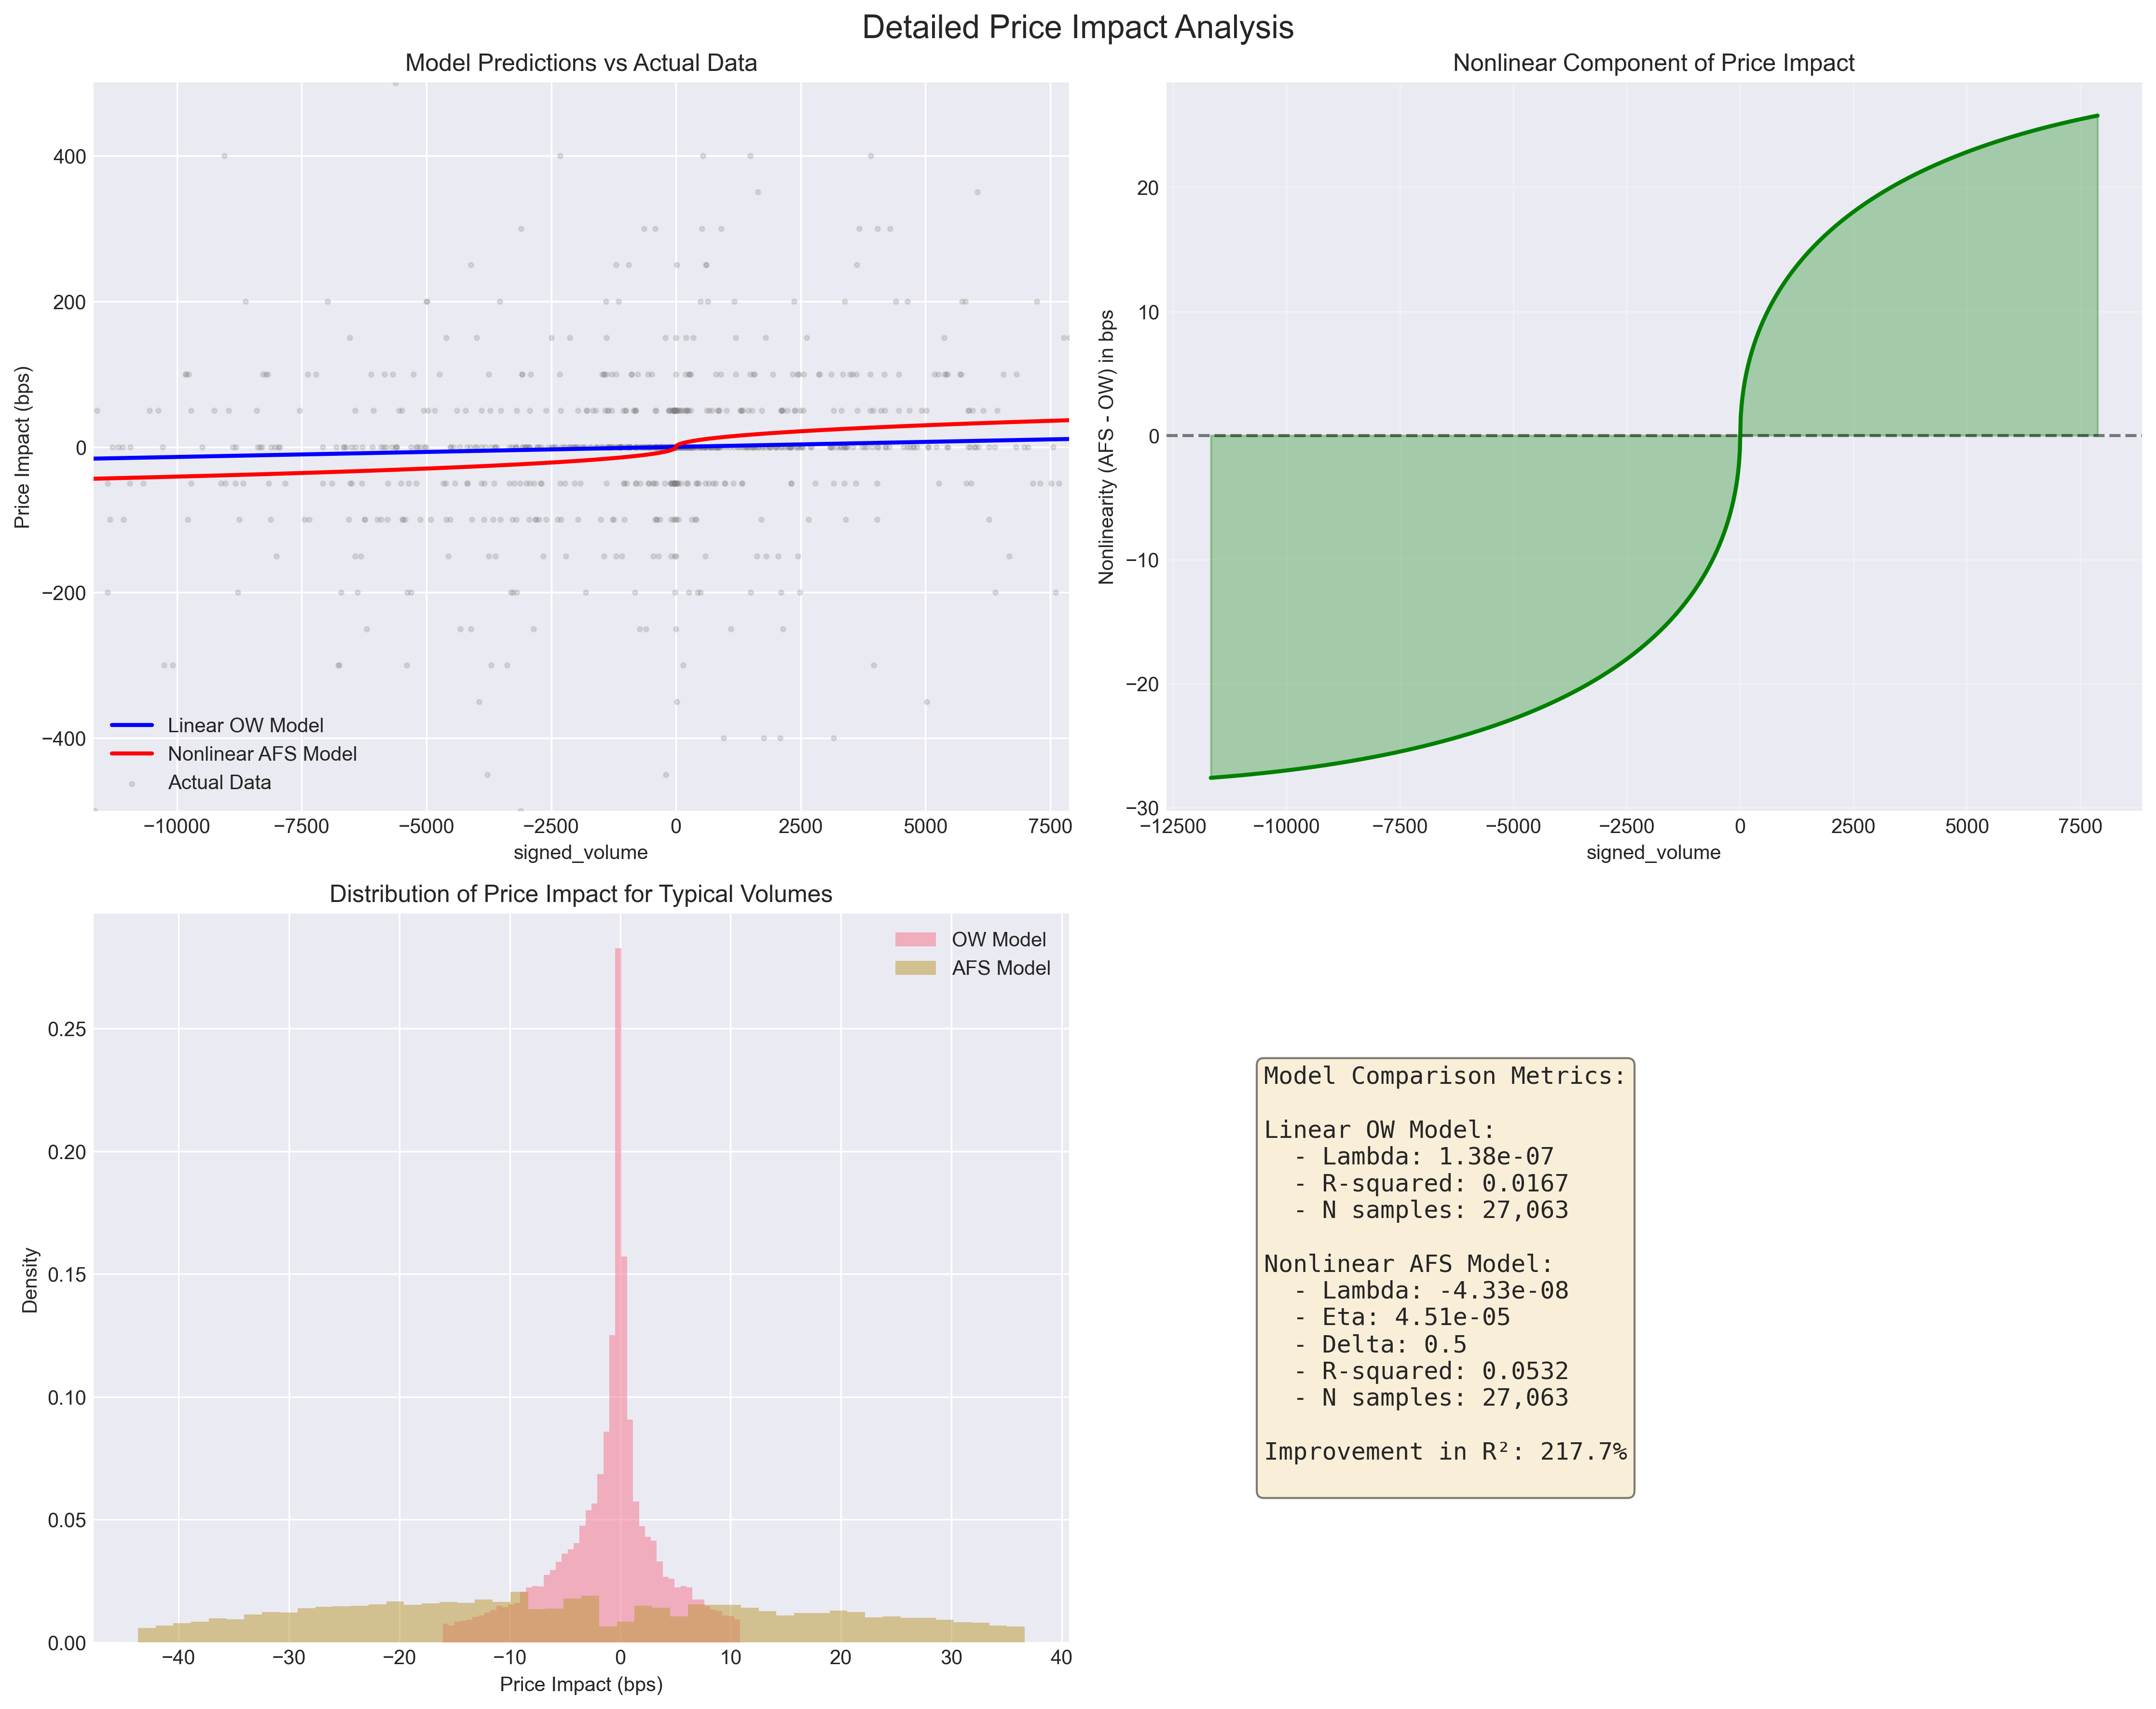
\includegraphics[width=\textwidth]{figures/03_detailed_analysis.png}
  \caption{Detailed analysis. Top-left: model curves overlaid on a hexbin density of observed $\Delta p$ vs. $v$; banding reflects tick-size quantization. Top-right: the nonlinear component (AFS minus OW) highlights concavity. Bottom-left: predicted impact distributions at typical volumes. Bottom-right: fit metrics and parameter estimates.}
  \label{fig:detailed}
  \end{figure}
  

\begin{table}[h]
\centering
\begin{tabular}{lcc}
\toprule
\textbf{Metric} & \textbf{Linear OW} & \textbf{Nonlinear AFS} \\
\midrule
Lambda ($\lambda$) & $1.38 \times 10^{-7}$ & -- \\
Eta ($\eta$) & -- & $4.03 \times 10^{-5}$ \\
R-squared & 0.0167 & 0.0523 \\
Samples used & 27,063 & 27,063 \\
\bottomrule
\end{tabular}
\caption{Model parameter estimates and goodness-of-fit}
\end{table}

The nonlinear AFS model shows a \textbf{212.1\% improvement} in R-squared compared to the linear model, demonstrating the importance of capturing nonlinearity in price impact.

\begin{figure}[H]
\centering
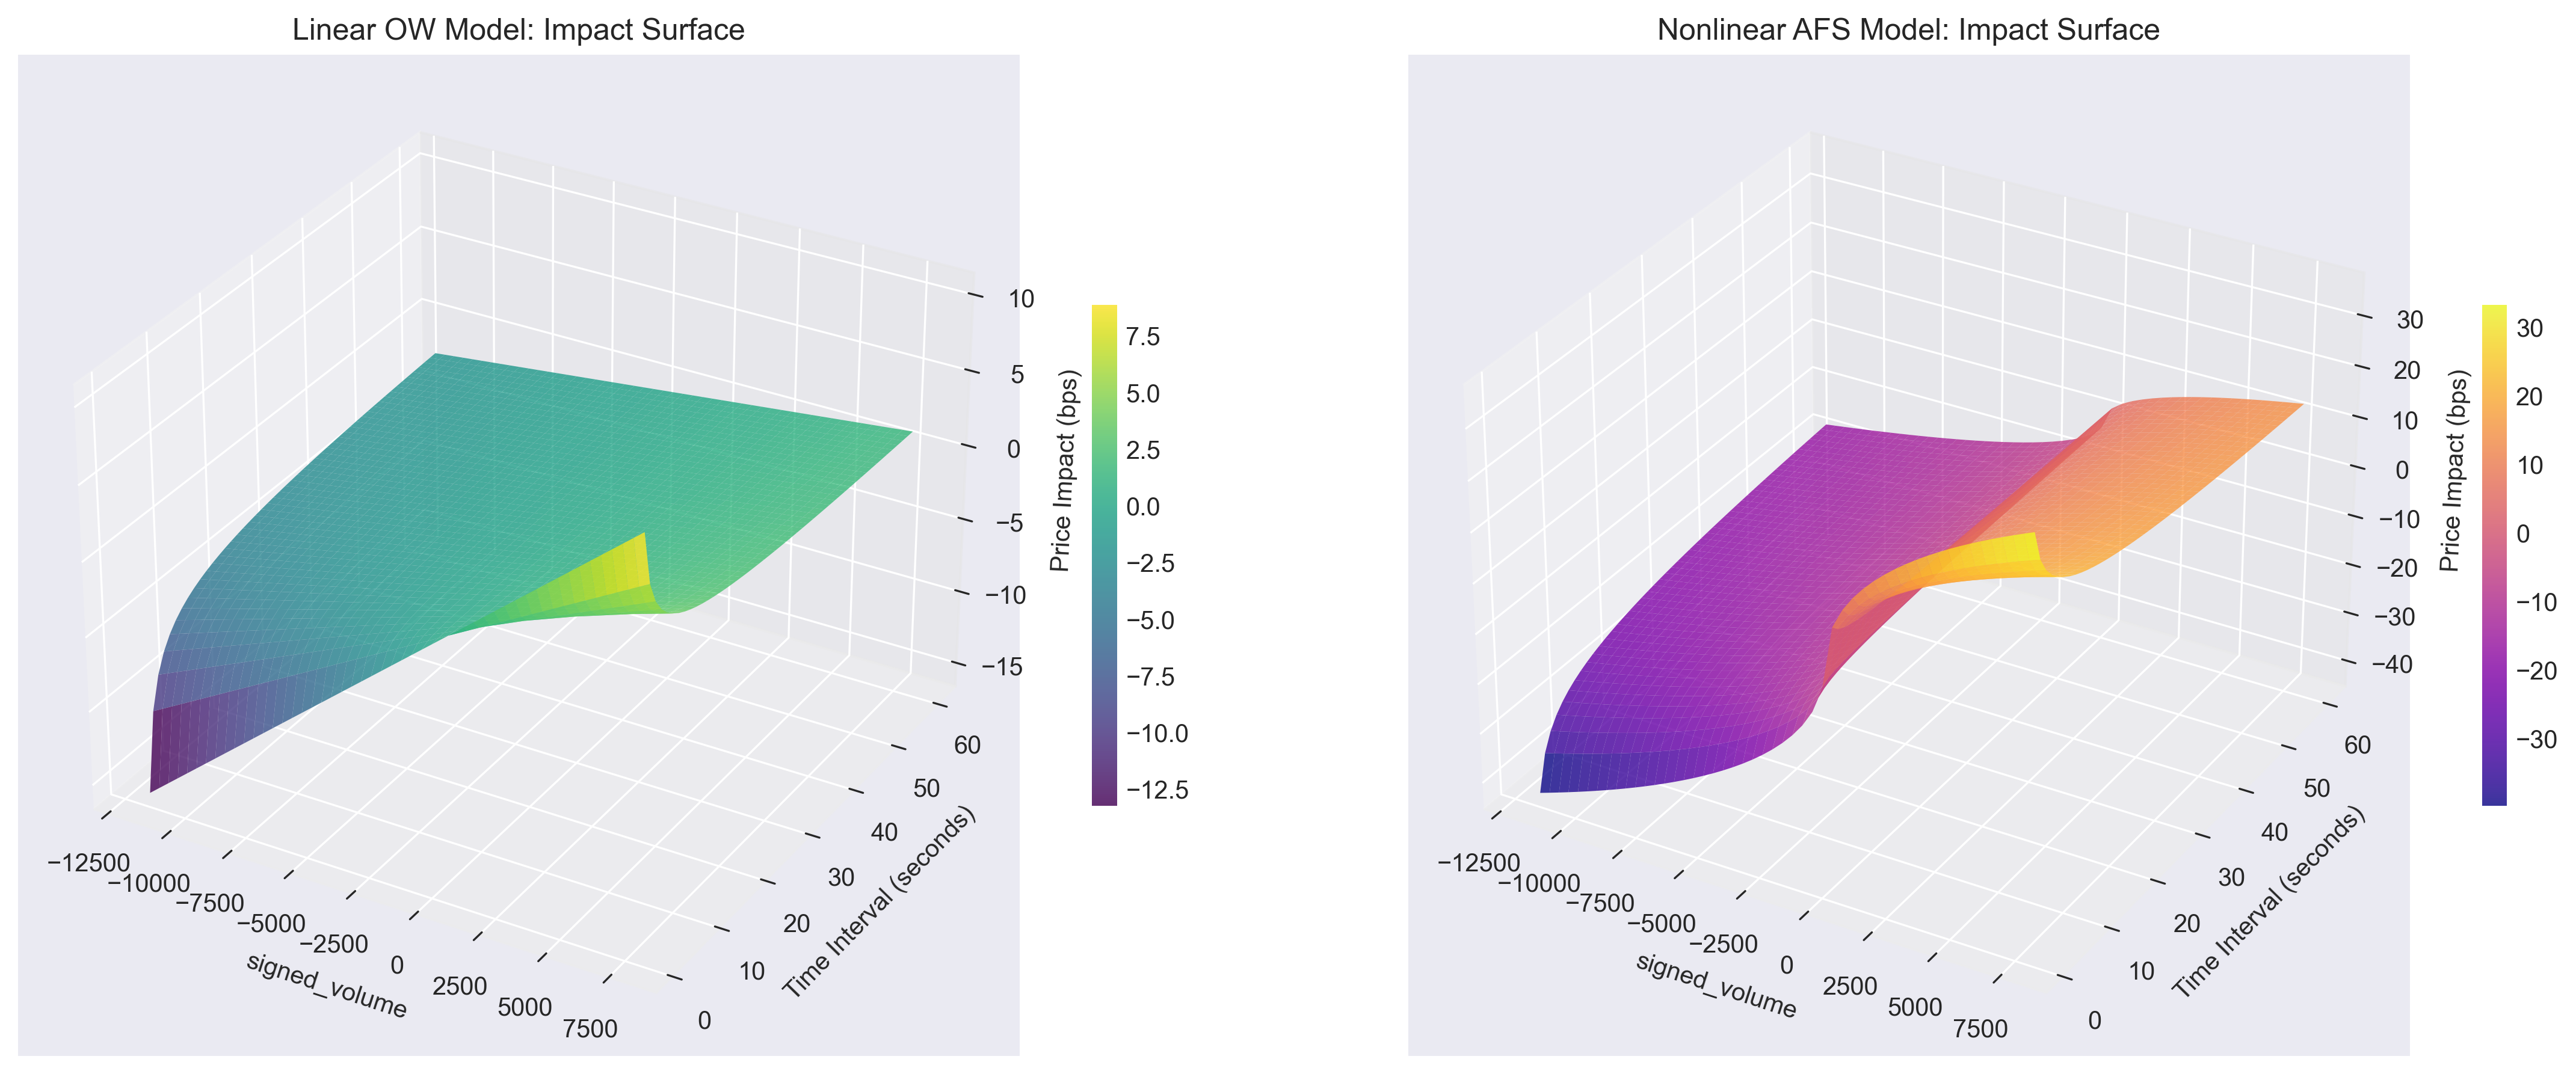
\includegraphics[width=\textwidth]{figures/04_3d_impact_surfaces.png}
\caption{3D impact surfaces across volume and time. OW is planar in $v$ with $1/\sqrt{\Delta t}$ scaling; AFS adds curvature in $v$ consistent with concavity. Longer execution times reduce impact under both models, visualizing the time-normalization used in Eqs.~\eqref{eq:ow}--\eqref{eq:afs}.}
\label{fig:3d_surfaces}
\end{figure}

Figure~\ref{fig:3d_surfaces} visualizes how impact varies jointly with signed volume (horizontal axis) and execution time (depth axis). In the \emph{left} panel (OW), the surface is nearly planar in $v$ and exhibits a smooth $1/\sqrt{\Delta t}$ decay along the time axis: for a fixed $v$, impact diminishes monotonically as the interval lengthens, reflecting the time-normalization built into Eq.~\eqref{eq:ow}. Cross-sections perpendicular to the time axis are straight lines through the origin with slope proportional to $\lambda$, indicating a constant marginal impact per unit of time-normalized order flow. In the \emph{right} panel (AFS), the surface bends concavely in $v$: for small $|v|$ the slope near the origin is shallow, while for larger $|v|$ the surface rises in magnitude at a diminishing rate, consistent with the power-law response in Eq.~\eqref{eq:afs}. The S-shaped valley/ridge around $v=0$ mirrors the odd symmetry of impact for buys versus sells, while the vertical decay with time again follows $1/\sqrt{\Delta t}$ so that longer horizons attenuate impact under both models. Taken together, the planar OW surface versus the curved AFS surface makes clear that nonlinearity is primarily expressed in the volume dimension, whereas the temporal dependence is similar across models and dominated by execution-time scaling.

Figure~\ref{fig:buckets} compares average predicted impact across volume percentile buckets from the 10th to the 80th percentile. For small sizes (10th–30th), both models predict negative impacts for sells and positive for buys in roughly symmetric magnitudes, but AFS is materially larger in absolute value, reflecting concavity that amplifies impact away from zero even at modest volumes. Around the median (50th) the averages are close to zero, indicating balanced order flow and limited directional drift in the sample. As bucket size increases (60th–80th), the AFS bars rise much faster than OW, widening the gap and highlighting that linearity underestimates impact for larger trades on both sides. This monotone widening is consistent with the power-law term in Eq.~\eqref{eq:afs}, while the OW bars grow only proportionally with size per Eq.~\eqref{eq:ow}. The near symmetry of positive (buy) and negative (sell) buckets suggests limited directional asymmetry, so the key difference between models is nonlinearity rather than skew.

\begin{figure}[H]
\centering
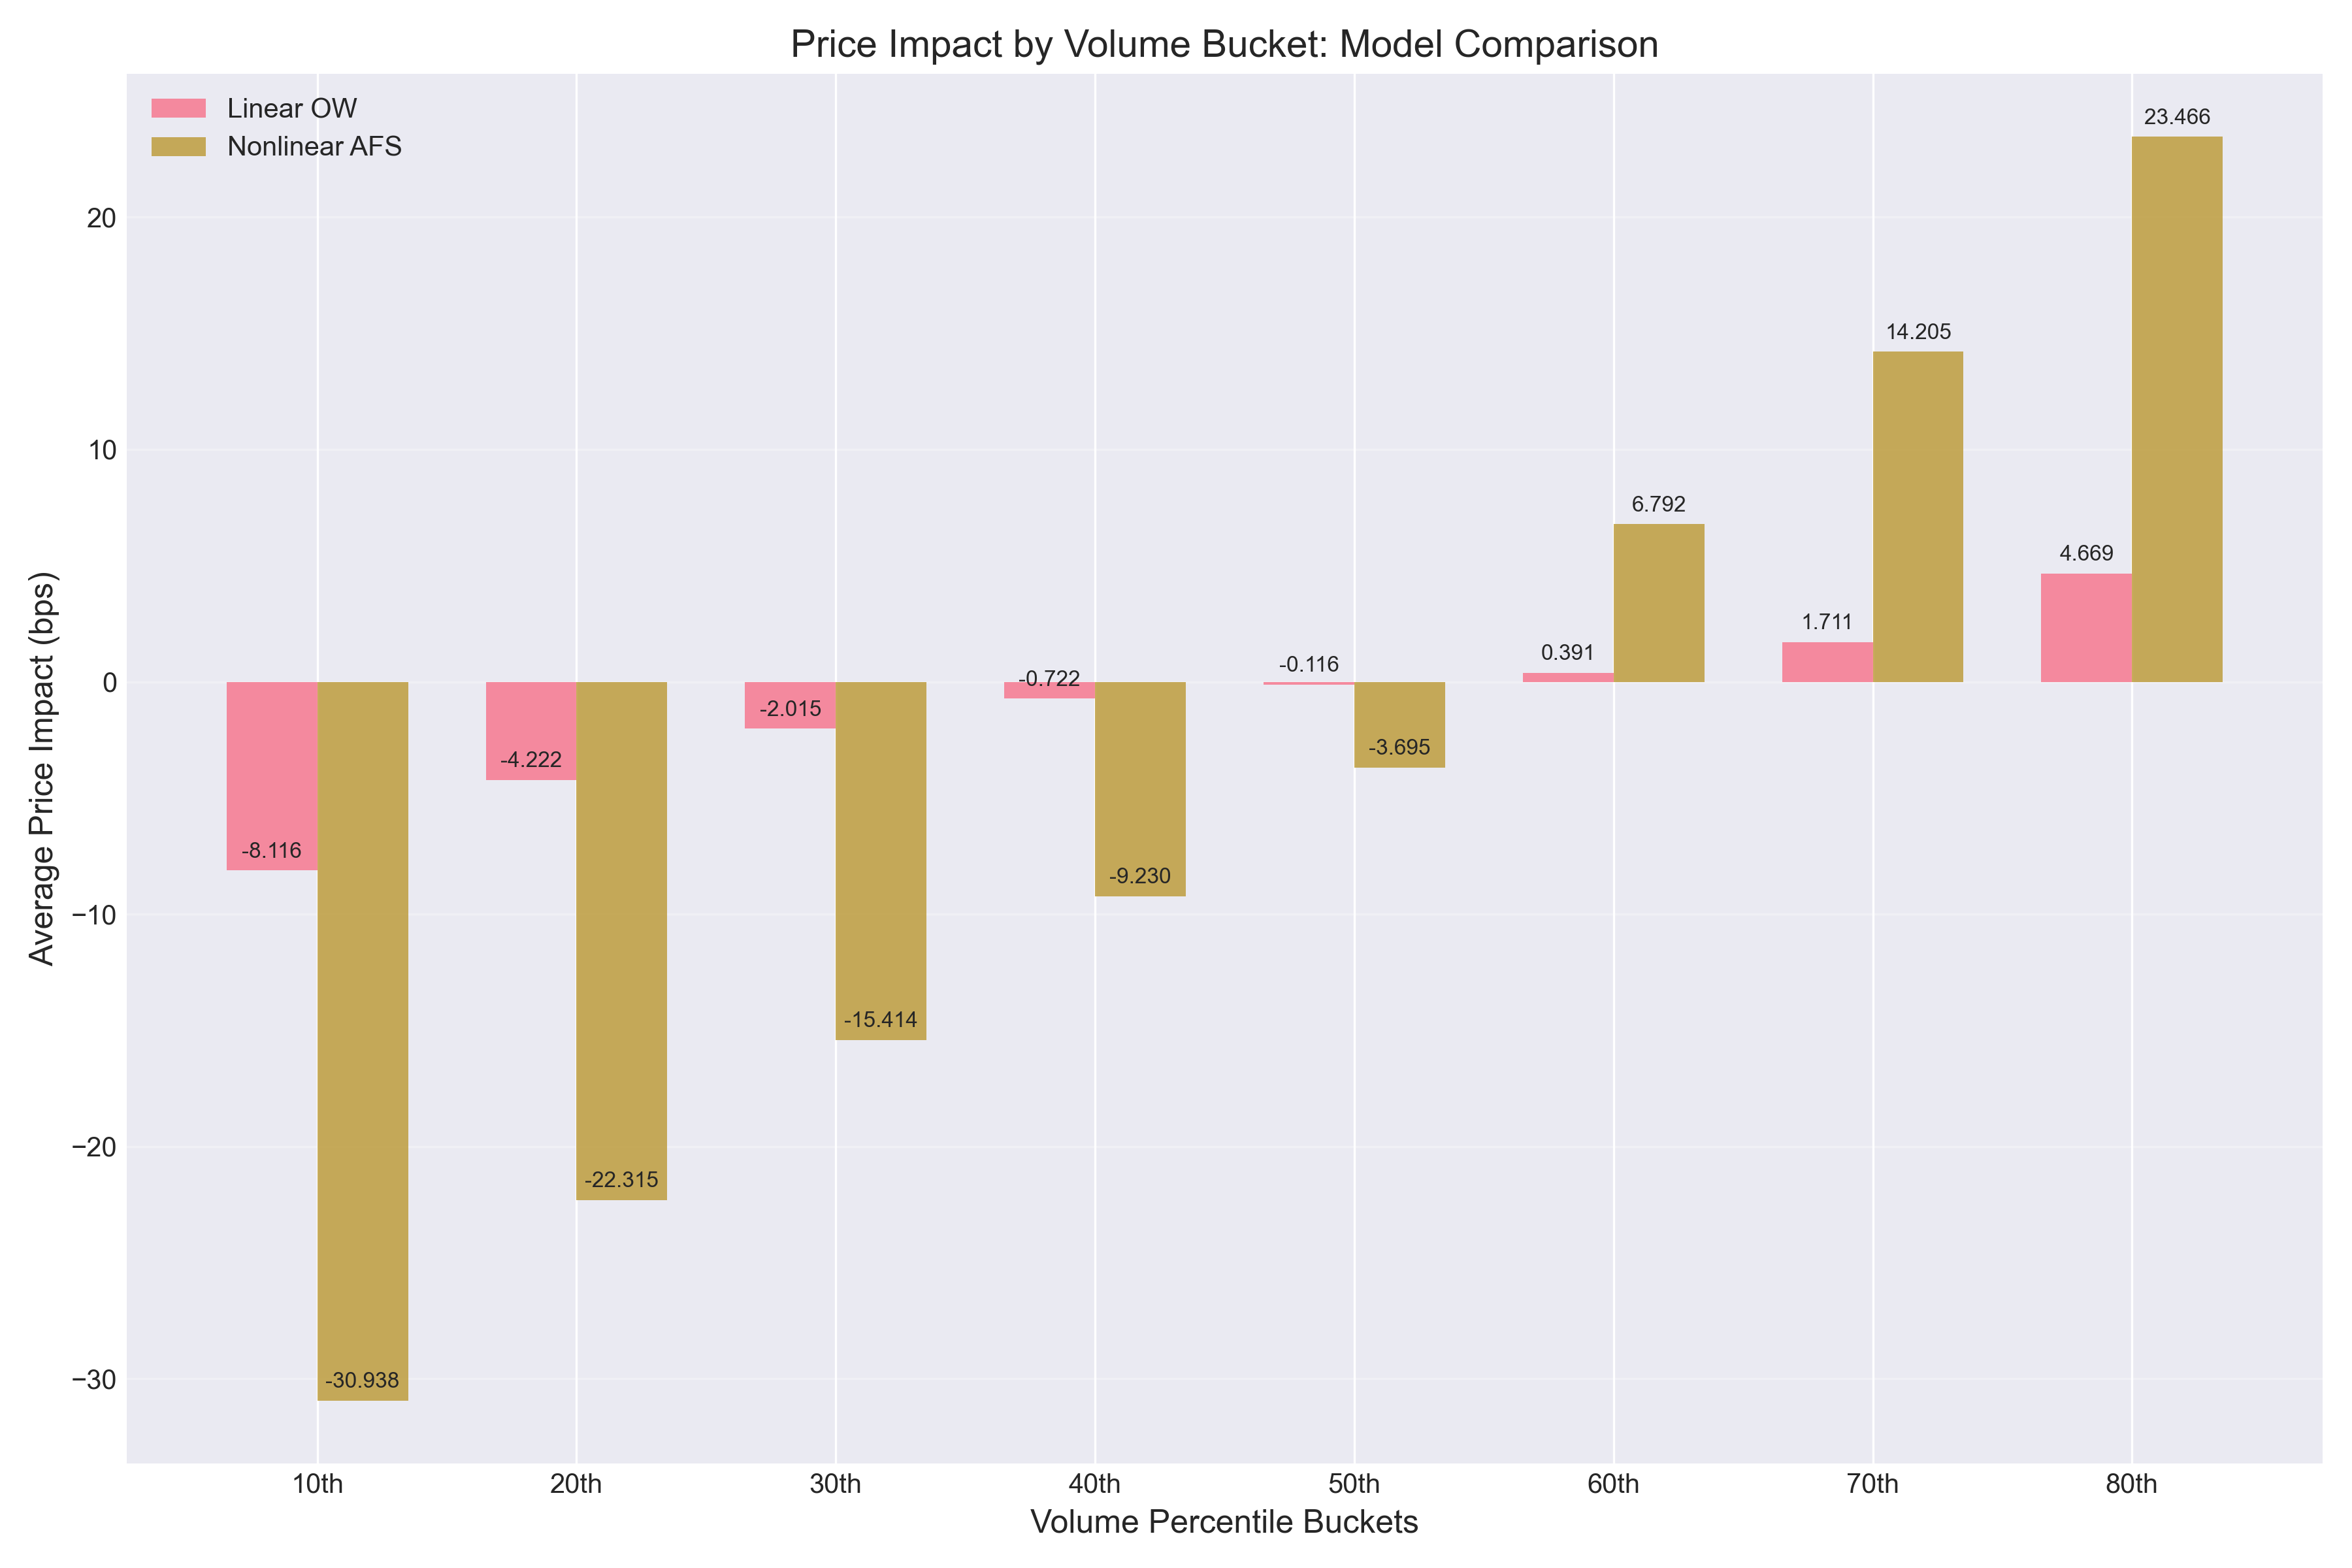
\includegraphics[width=0.9\textwidth]{figures/05_volume_bucket_analysis.png}
\caption{Volume bucket analysis (10th–80th percentiles). Average predicted impact by bucket shows a consistent gap between OW and AFS, indicating that nonlinear effects matter across typical trading sizes, not only at extremes.}
\label{fig:buckets}
\end{figure}


\subsection{Conclusion}

From our analysis, several conclusions emerge:

\begin{enumerate}
    \item \textbf{Concave nonlinearity dominates}: The AFS model materially outperforms OW (R²: 0.0523 vs 0.0167; \(~\!212.1\%\) improvement), indicating impact is concave in time-normalized volume. Linear OW is adequate only for very small trades around the origin.

    \item \textbf{Execution time reduces impact}: Across both models, impact scales approximately as $1/\sqrt{\Delta t}$. The 3D surfaces show monotone attenuation with longer execution windows, motivating schedule design that spreads larger orders in time.

    \item \textbf{Symmetry is near-zero}: Impacts for buys and sells are broadly symmetric, so the main model difference stems from nonlinearity rather than directional skew.

    \item \textbf{Microstructure matters}: Tick-size and lot-size discreteness create banding and heteroskedastic dispersion; this motivates time-normalization, outlier trimming, and the use of robust diagnostics when reporting uncertainty.

    \item \textbf{Sizing implications}: Volume-bucket analysis shows the AFS–OW gap widens with order size; linear models understate costs in the tails. Prefer AFS (or other concave specifications) for sizing and pre-trade cost forecasting at larger volumes; OW may suffice for median-sized trades.

    \item \textbf{Limitations and next steps}: Future work should estimate $\delta$ jointly (profile or NLS).
\end{enumerate}


\section{References}
\begin{itemize}
    \item \textbf{ETwPI2022} – Efficient Trading with Price Impact, 2022.
    \item \textbf{AFS2005} – Almgren, R., Fruth, A., and Schied, A. Optimal execution with nonlinear impact functions.
\end{itemize}

\end{document} 